\begin{figure}[tb]
    \centering
    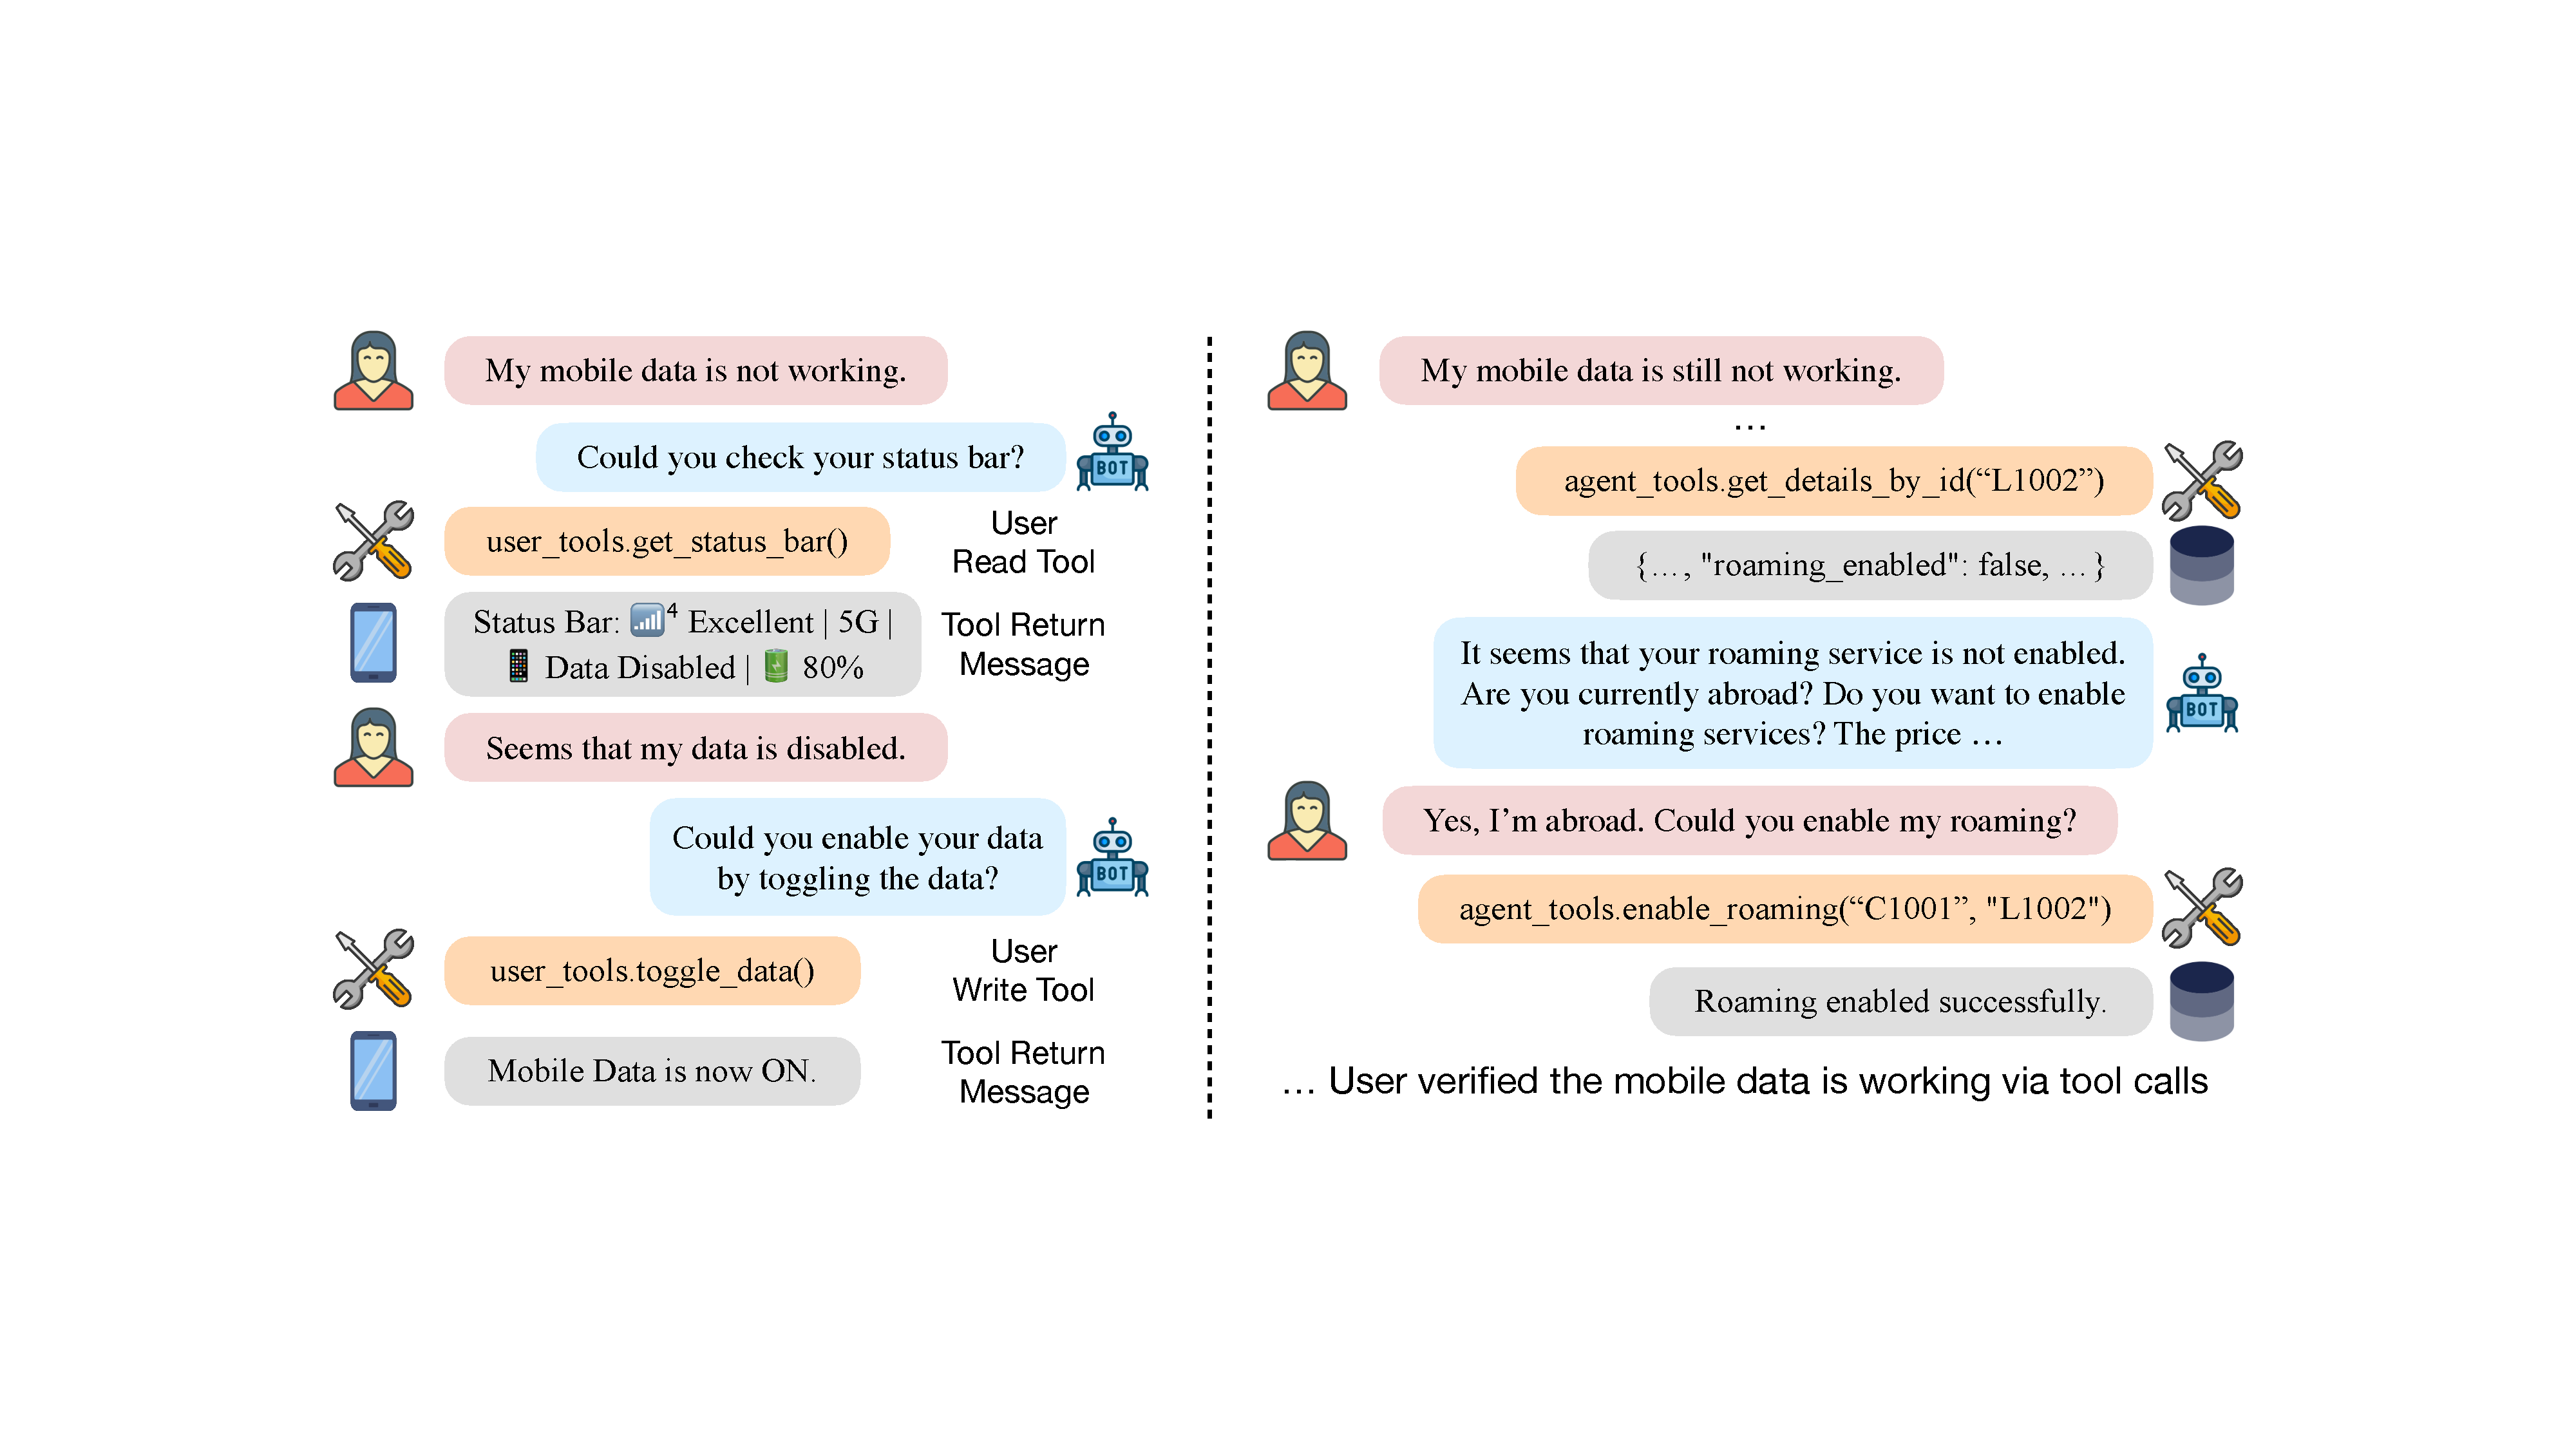
\includegraphics[width=0.99\textwidth,trim=240 240 240 240,clip]{figures/raw/traj.pdf}
    \vspace{-0.5em}
    \caption{An example agent-user interaction trajectory ($\gS_{history}$) of \bench in the \telecom domain. By controlling the implementation of the user tools (the mocked phone), we can reliably simulate the user's response to agent's actionable instructions like ``checking the status bar'' and ``toggling data'' based on the underlying database state. On the right half, we show the possibility of modeling the impact of agent's tool calls on the user's database state, where the roaming service for the user is enabled on the agent's end and therefore allows the user's phone to roam.}
    \label{fig:traj}
\end{figure}
